\documentclass[journal,12pt,twocolumn]{IEEEtran}

\usepackage{setspace}
\usepackage{gensymb}
\singlespacing
\usepackage[cmex10]{amsmath}

\usepackage{amsthm}

\usepackage{mathrsfs}
\usepackage{txfonts}
\usepackage{stfloats}
\usepackage{bm}
\usepackage{cite}
\usepackage{cases}
\usepackage{subfig}

\usepackage{longtable}
\usepackage{multirow}

\usepackage{enumitem}
\usepackage{mathtools}
\usepackage{steinmetz}
\usepackage{tikz}
\usepackage{circuitikz}
\usepackage{verbatim}
\usepackage{tfrupee}
\usepackage[breaklinks=true]{hyperref}
\usepackage{graphicx}
\usepackage{tkz-euclide}

\usetikzlibrary{calc,math}
\usepackage{listings}
    \usepackage{color}                                            %%
    \usepackage{array}                                            %%
    \usepackage{longtable}                                        %%
    \usepackage{calc}                                             %%
    \usepackage{multirow}                                         %%
    \usepackage{hhline}                                           %%
    \usepackage{ifthen}                                           %%
    \usepackage{lscape}     
\usepackage{multicol}
\usepackage{chngcntr}

\DeclareMathOperator*{\Res}{Res}

\renewcommand\thesection{\arabic{section}}
\renewcommand\thesubsection{\thesection.\arabic{subsection}}
\renewcommand\thesubsubsection{\thesubsection.\arabic{subsubsection}}

\renewcommand\thesectiondis{\arabic{section}}
\renewcommand\thesubsectiondis{\thesectiondis.\arabic{subsection}}
\renewcommand\thesubsubsectiondis{\thesubsectiondis.\arabic{subsubsection}}


\hyphenation{op-tical net-works semi-conduc-tor}
\def\inputGnumericTable{}                                 %%

\lstset{
%language=C,
frame=single, 
breaklines=true,
columns=fullflexible
}
\begin{document}

\newcommand{\BEQA}{\begin{eqnarray}}
\newcommand{\EEQA}{\end{eqnarray}}
\newcommand{\define}{\stackrel{\triangle}{=}}
\bibliographystyle{IEEEtran}
\raggedbottom
\setlength{\parindent}{0pt}
\providecommand{\mbf}{\mathbf}
\providecommand{\pr}[1]{\ensuremath{\Pr\left(#1\right)}}
\providecommand{\qfunc}[1]{\ensuremath{Q\left(#1\right)}}
\providecommand{\sbrak}[1]{\ensuremath{{}\left[#1\right]}}
\providecommand{\lsbrak}[1]{\ensuremath{{}\left[#1\right.}}
\providecommand{\rsbrak}[1]{\ensuremath{{}\left.#1\right]}}
\providecommand{\brak}[1]{\ensuremath{\left(#1\right)}}
\providecommand{\lbrak}[1]{\ensuremath{\left(#1\right.}}
\providecommand{\rbrak}[1]{\ensuremath{\left.#1\right)}}
\providecommand{\cbrak}[1]{\ensuremath{\left\{#1\right\}}}
\providecommand{\lcbrak}[1]{\ensuremath{\left\{#1\right.}}
\providecommand{\rcbrak}[1]{\ensuremath{\left.#1\right\}}}
\theoremstyle{remark}
\newtheorem{rem}{Remark}
\newcommand{\sgn}{\mathop{\mathrm{sgn}}}
\providecommand{\abs}[1]{\vert#1\vert}
\providecommand{\res}[1]{\Res\displaylimits_{#1}} 
\providecommand{\norm}[1]{\lVert#1\rVert}
%\providecommand{\norm}[1]{\lVert#1\rVert}
\providecommand{\mtx}[1]{\mathbf{#1}}
\providecommand{\mean}[1]{E[ #1 ]}
\providecommand{\fourier}{\overset{\mathcal{F}}{ \rightleftharpoons}}
%\providecommand{\hilbert}{\overset{\mathcal{H}}{ \rightleftharpoons}}
\providecommand{\system}{\overset{\mathcal{H}}{ \longleftrightarrow}}
	%\newcommand{\solution}[2]{\textbf{Solution:}{#1}}
\newcommand{\solution}{\noindent \textbf{Solution: }}
\newcommand{\cosec}{\,\text{cosec}\,}
\providecommand{\dec}[2]{\ensuremath{\overset{#1}{\underset{#2}{\gtrless}}}}
\newcommand{\myvec}[1]{\ensuremath{\begin{pmatrix}#1\end{pmatrix}}}
\newcommand{\mydet}[1]{\ensuremath{\begin{vmatrix}#1\end{vmatrix}}}
\numberwithin{equation}{subsection}
\makeatletter
\@addtoreset{figure}{problem}
\makeatother
\let\StandardTheFigure\thefigure
\let\vec\mathbf
\renewcommand{\thefigure}{\theproblem}
\def\putbox#1#2#3{\makebox[0in][l]{\makebox[#1][l]{}\raisebox{\baselineskip}[0in][0in]{\raisebox{#2}[0in][0in]{#3}}}}
     \def\rightbox#1{\makebox[0in][r]{#1}}
     \def\centbox#1{\makebox[0in]{#1}}
     \def\topbox#1{\raisebox{-\baselineskip}[0in][0in]{#1}}
     \def\midbox#1{\raisebox{-0.5\baselineskip}[0in][0in]{#1}}
\vspace{3cm}
\title{Assignment 3}
\author{Digjoy Nandi - AI20BTECH11007}
\maketitle
\newpage
\bigskip
\renewcommand{\thefigure}{\theenumi}
\renewcommand{\thetable}{\theenumi}
Download all python codes from 
\begin{lstlisting}

\end{lstlisting}
%
and latex codes from 
%
\begin{lstlisting}

\end{lstlisting}
\section{Problem}
(Gate MA - 2016 Q.47) Let $X_{1}$ be	an	exponential	random	variable with mean 1 and $X_{2}$ a gamma	random variable	with mean 2	and	variance 2.	If $X_{1}$ and $X_{2}$ are independently	distributed, then $\pr{X_1 < X_2}$ is equal	to ..........	
\section{Solution}
We know that,
\begin{align}
    f(X_1) = 
    \begin{cases}
    0   & x < 0\\
    \frac{\exp{(\frac{{-X_1}}{\beta}})}{\beta} & 0\le x < \infty\\
    \end{cases}
\end{align}
Given, $E(X_1)=\beta=1$\\
Therefore,
\begin{align}
    f(X_1) = 
    \begin{cases}
    0   & x < 0\\
    \exp{(-X_1)} & 0\le x < \infty\\
    \end{cases}
\end{align}
We know that,
\begin{align}
    f(X_2) = 
    \begin{cases}
    0   & x < 0\\
    \frac{X_{2}^{\alpha-1}\exp{(\frac{-X_2}{\beta})}}{\beta^{\alpha}\Gamma(\alpha)} & 0\le x < \infty\\
    \end{cases}
\end{align}
Given, 
\begin{equation}\label{eq:2.0.4}
    E(X_2)=\alpha \beta =2 
\end{equation}
\begin{equation}\label{eq:2.0.5}
    V(X_2)=\alpha \beta^{2}=2 
\end{equation}

Solving \ref{eq:2.0.4} and \ref{eq:2.0.5}, we get,
$\alpha=2$, $\beta=1$ and $\Gamma(2)=1$\\
Therefore,
\begin{align}
    f(X_2) = 
    \begin{cases}
    0   & x < 0\\
    X_2\exp{(-X_2)} & 0\le x < \infty\\
    \end{cases}
\end{align}

\begin{figure}[!ht]
\centering
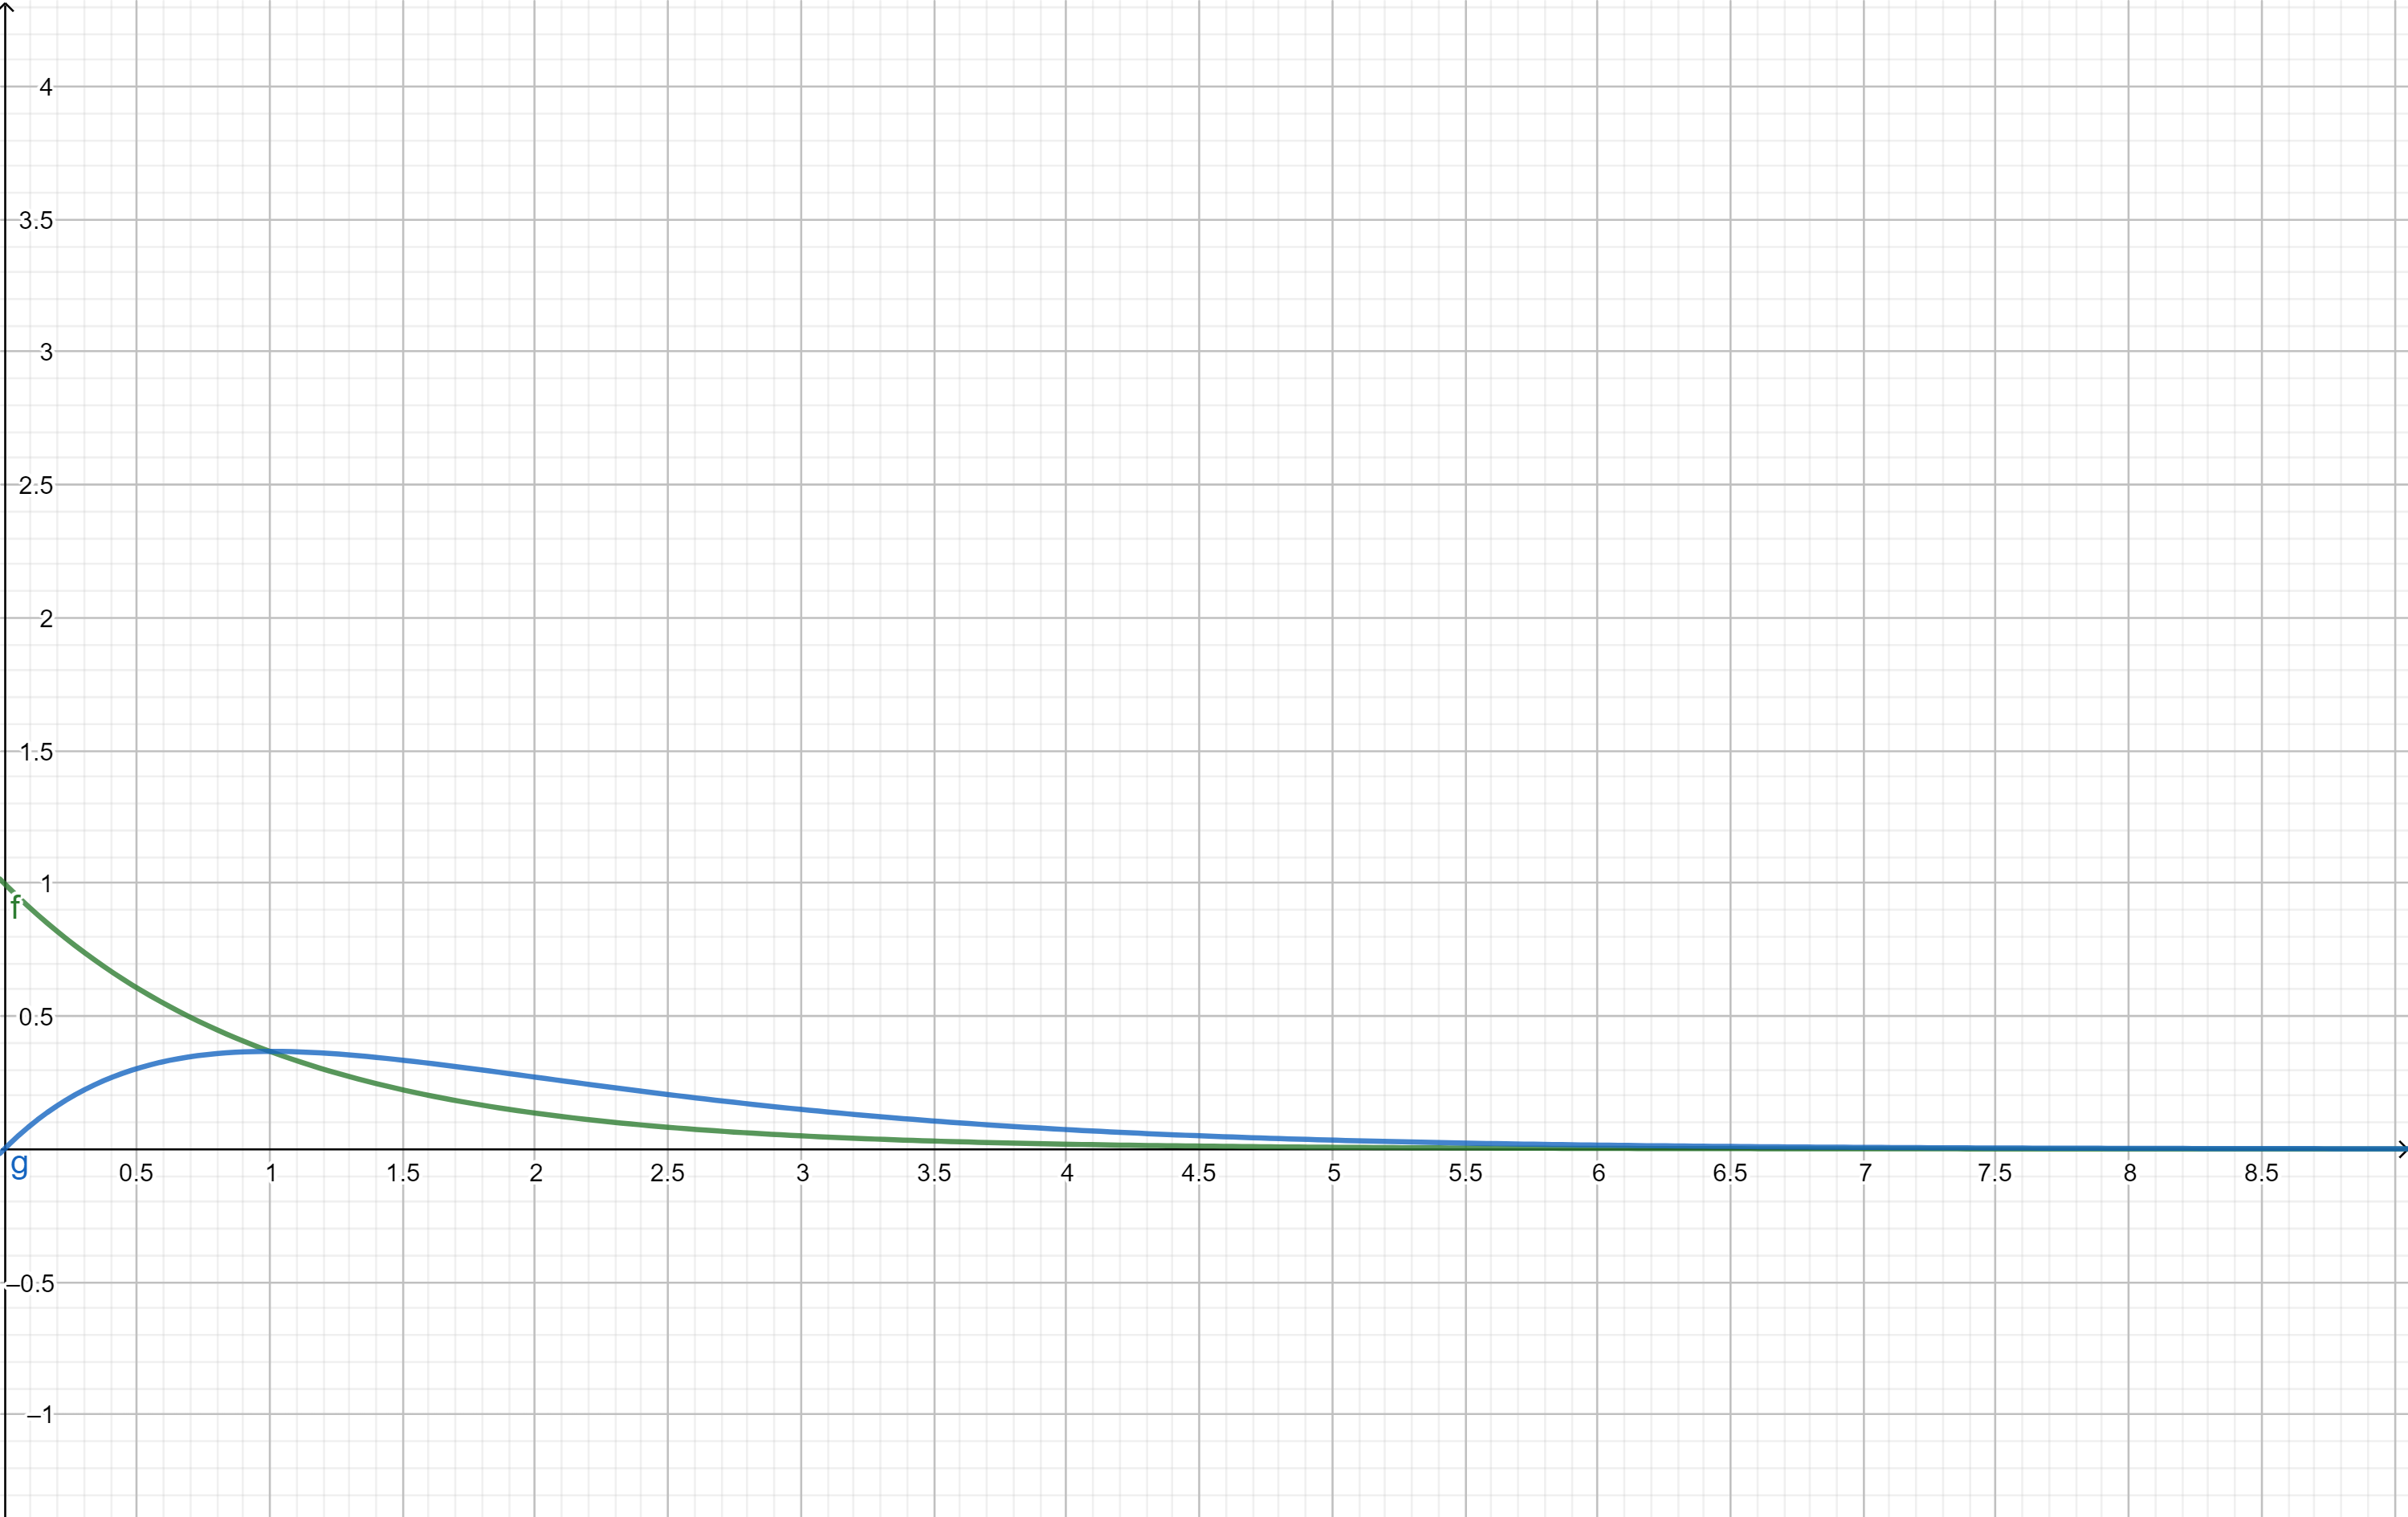
\includegraphics[width=\columnwidth]{figure.png}
\caption{Probability Distribution of $(X_1, X_2)$}
\end{figure}

Alternately, we have CDF of $X_1$ and $X_2$ given by 
\begin{align}
    F_{X_1}(x) = 
    \begin{cases}
     0   & x < 0\\
    1-\exp{(-x)} & 0\le x < \infty\\
    \end{cases}
\end{align}
\begin{align}
    F_{X_2}(x) = 
    \begin{cases}
    0   & x < 0\\
    1-(x+1)\exp{(-x)} & 0\le x < \infty\\
    \end{cases}
\end{align}

Thus 
\begin{align}
    \pr{X_1\le X_2} &= \int_{-\infty}^{\infty} F_{X_1}(x)f(X_2)dX\\
                &= \int_0^\infty -\exp{(-x)}x\exp{(-x)}dx\\
                &= \cfrac{3}{4}
\end{align}
\end{document}
